\usepackage[english]{babel}
\usepackage[utf8]{inputenc}
\usepackage[T1]{fontenc}
\usepackage{helvet}
\usepackage{nimbusmononarrow}
\usepackage{euler}
\usepackage{tikz}
\usepackage{listings}
\usepackage{relsize}
\usepackage{booktabs}

\usetikzlibrary{arrows}
\usetikzlibrary{backgrounds}
\usetikzlibrary{chains}
\usetikzlibrary{fit}
\usetikzlibrary{positioning}
\usetikzlibrary{scopes}
\usetikzlibrary{trees}
\usetikzlibrary{automata}
\usetikzlibrary{positioning}
\usetikzlibrary{shapes.multipart}

\usetheme{boxes}
%\useoutertheme{essential}
\usecolortheme{seagull}
\usefonttheme{structurebold}
\setbeamertemplate{navigation symbols}{}
\setbeamertemplate{frametitle}
{
	\begin{centering}
		\vspace{1.5em}
		\LARGE
    \insertframetitle
    \par
    \vspace{0.5em}
  \end{centering}
}
\setbeamerfont{title}{size=\huge}
\setbeamerfont{subtitle}{size=\Large}

\lstset{basicstyle=\ttfamily\scriptsize}
\newcommand{\cinput}[1]{\lstinputlisting[language=C,basicstyle=\ttfamily]{#1}}
\newcommand{\cinline}[1]{\lstinline[language=C,basicstyle=\ttfamily]!#1!}
\newcommand{\cppinput}[1]{\lstinputlisting[language=C++,basicstyle=\ttfamily]{#1}}
\newcommand{\cppinline}[1]{\lstinline[language=C++,basicstyle=\ttfamily]!#1!}
\newcommand{\llvminput}[1]{\lstinputlisting[language=LLVM,basicstyle=\ttfamily]{#1}}
\newcommand{\llvminline}[1]{\lstinline[language=LLVM,basicstyle=\ttfamily]!#1!}
\lstdefinelanguage{LLVM}%
  {morekeywords={define,declare,global,constant,internal,external,private,%
      linkonce,linkonce_odr,weak,weak_odr,appending,common,extern_weak,%
      thread_local,dllimport,dllexport,hidden,protected,default,except,deplibs,%
      volatile,fastcc,coldcc,cc,ccc,x86_stdcallcc,x86_fastcallcc,ptx_kernel,%
      ptx_device,signext,zeroext,inreg,sret,nounwind,noreturn,nocapture,byval,%
      nest,readnone,readonly,noalias,uwtable,inlinehint,noinline,alwaysinline,%
      optsize,ssp,sspreq,noredzone,noimplicitfloat,naked,alignstack,module,asm,%
      align,tail,to,addrspace,section,alias,sideeffect,c,gc,target,datalayout,%
      triple,blockaddress},%
  morekeywords=[2]{add,fadd,sub,fsub,mul,fmul,sdiv,udiv,fdiv,srem,urem,frem,%
     and,or,xor,icmp,fcmp,eq,ne,ugt,uge,ult,ule,sgt,sge,slt,sle,oeq,ogt,oge,%
     olt,ole,one,ord,ueq,ugt,uge,ult,ule,une,uno,nuw,nsw,exact,inbounds,phi,%
     call,select,shl,lshr,ashr,va_arg,trunc,zext,sext,fptrunc,fpext,fptoui,%
     fptosi,uitofp,sitofp,ptrtoint,inttoptr,bitcast,ret,br,indirectbr,switch,%
     invoke,unwind,unreachable,malloc,alloca,free,load,store,getelementptr,%
     extractelement,insertelement,shufflevector,extractvalue,insertvalue},%
  sensitive=t,%
  morestring=[b]",%
  morecomment=[l];%
  }[keywords,comments,strings]


\author{Daniele Cattaneo}
\institute{Politecnico di Milano}
\date{\DATE}
\title{The LLVM compiler framework}
\subtitle{Exploring LLVM}
\newcommand{\customdata}{Daniele Cattaneo <daniele.cattaneo@polimi.it>}

\AtBeginSection[]
{
\begin{frame}{Contents}
\tableofcontents[currentsection,subsectionstyle=show/shaded/hide]
\end{frame}
}

\AtBeginSubsection[]
{
\begin{frame}{Contents}
\tableofcontents[currentsection,subsectionstyle=show/shaded/hide]
\end{frame}
}

\begin{document}


\begin{frame}
\maketitle
\begin{center}
\itshape\scriptsize
These slides were originally written by
Michele Scandale, Ettore Speziale and Stefano Cherubin for the
``Code Transformation and Optimization'' course.
\end{center}
\end{frame}


% !TEX root = 02.tex

\section{Documentation}
\begin{frame}[t]{LLVM official documentation}
  \begin{center}
    \begin{Huge}
      \vfill
      \url{llvm.org/docs}
      \vfill
    \end{Huge}
  \end{center}
\end{frame}
%--- Next Frame ---%

\begin{frame}[t]{A lot of documentation...}
  \url{llvm.org/docs} mentions:
  \begin{itemize}
    \item \texttt{\ 5} references about \textit{Design \& Overview}
    \item \texttt{23} references about \textit{User Guides}
    \item \texttt{15} references about \textit{Programming Documentation}
    \item \texttt{42} references about \textit{Subsystem Documentation}
    \item \texttt{\ 9} references about \textit{Development Process Documentation}
    \item \texttt{\ 5} Mailing Lists
    \item \texttt{\ 5} IRC bots
  \end{itemize}
  \vfill
  Most of the above references are OUT-OF-DATE.
  \vfill
  You probably need documentation about the documentation itself.
  \vfill
\end{frame}
%--- Next Frame ---%

\begin{frame}[t]{Essential documentation}
  \begin{description}
    \item[Intro to LLVM] \cite{LOCAL:www/llvmIntro}
          gives a quick and clear introduction to the compiler infrastructure.
          It is mostly up-to-date.\footnote{at the time I am writing}
    \vfill
    \item[Writing an LLVM pass] \cite{LOCAL:www/llvmWritingAPass}
          explains step by step how to implement a Pass
          for those who never did anything like that.
          We will see this tutorial later in the course.
    \vfill
    \item[Doxygen] \cite{LOCAL:www/llvmDoxygen}
          \textit{The best code documentation is the code itself.}
          Sometimes the generated doxygen documentation is enough.
          It also contains links to the web version of the source code.
          It is updated to the latest development branch.
          Please refer to github branches for the documentation about the stable versions.
    \vfill
    \item[llvm-dev] Mailing List. Last resource: ask other developers.
          Warning: 24/7 many people are posting in this ML.
  \end{description}
\end{frame}

% !TEX root = 02.tex

\section{Normalization Passes}
\begin{frame}{Canonicalize Pass Input}
We will see the following passes:

\begin{table}
\centering
\begin{tabular}{cc}
\toprule

\multicolumn{1}{c}{\textbf{Pass}}    &
\multicolumn{1}{c}{\textbf{Switch}} \\

\midrule

Variable promotion  &
\texttt{mem2reg}   \\

Loop simplify           &
\texttt{loop-simplify} \\

Loop-closed SSA  &
\texttt{lcssa}  \\

Induction variable simplification  &
\texttt{indvars}                  \\

\bottomrule
\end{tabular}
\end{table}

They are \alert{normalization} passes:

\begin{itemize}
\item put data into a canonical form
\end{itemize}
\end{frame}

\begin{frame}{Variable Promotion}
One of the most difficult things in compiler is:

\begin{itemize}
\item considering memory accesses
\end{itemize}

\vfill
\begin{block}{Plain SAXPY}
\centering
\llvminput{snippet/plain-saxpy.ll}
\end{block}
\end{frame}

\begin{frame}{Variable Promotion}{Simplifying Representation}
In the SAXPY kernel some \llvminline{alloca} are generated:

\begin{itemize}
\item represent \alert{local variables}~\footnote{Arguments are considered local variables}
\end{itemize}

\vfill
They are generated due to compiler \alert{conservative} approach:

\begin{itemize}
\item maybe some instruction can take the addresses of such variables, hence a
      memory location is needed
\end{itemize}

\vfill
Complex representations makes hard performing further actions:

\begin{itemize}
\item suppose you want to compute \cinline{a * x + y} using only one
      instruction~\footnote{e.g. FMA4}
\item hard to detect due to \llvminline{load} and \llvminline{store}
\end{itemize}
\end{frame}

\begin{frame}{Variable Promotion}{Using Memory Only When Necessary}
To limit the number of instruction accessing memory:

\begin{itemize}
\item we need to eliminate \llvminline{load} and \llvminline{store}
\item achieved by \alert{promoting} variables from memory to registers
\end{itemize}

\vfill
Inside LLVM SSA-based representation:

\begin{description}
\item[memory] Stack allocations --
              e.g \llvminline{\%1 = alloca float, align 4}
\item[register] SSA variables -- e.g. \llvminline{\%a}
\end{description}

\vfill
The \texttt{mem2reg} pass focus on:

\begin{itemize}
\item eliminating \llvminline{alloca} with only \llvminline{load} and
      \llvminline{store} uses
\end{itemize}

Also available as utility:

\begin{itemize}
\item \cppinline{llvm::PromoteMemToReg}\footnote{see lib/Transforms/Utils/PromoteMemoryToRegister.cpp}
\end{itemize}
\end{frame}

\begin{frame}{Variable Promotion}{Example on simplified code}
\begin{columns}[t]
\column{.45\textwidth}
\begin{block}{Starting Point}
\centering
\llvminput{snippet/saxpy.ll}
\end{block}

Copy propagation performed transparently by the compiler

\column{.45\textwidth}
\begin{block}{Promoting \llvminline{alloca}}
\centering
\llvminput{snippet/mem2reg-saxpy.ll}
\end{block}

\begin{block}{After Copy-propagation}
\centering
\llvminput{snippet/mem2reg-copy-saxpy.ll}
\end{block}

\end{columns}
\end{frame}

\begin{frame}{Loops}
Different kind of loops:

\begin{columns}[t]
\column{.30\textwidth}
\begin{block}{\cinline{do}-\cinline{while} Loops}
\centering

% do-while-loop.tex: do-while loop shape.

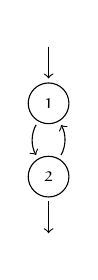
\begin{tikzpicture}
[
  every node/.style={
    font=\tiny
  },
  every initial by arrow/.style={
    shorten >=.5mm
  },
  every accepting by arrow/.style={
    shorten <=.5mm
  },
  entry above/.style={
    initial above,
    initial text=
  },
  exit below/.style={
    accepting below
  },
  bb/.style={
    circle,
    draw
  },
  tip/.style={
    shorten <=.5mm,
    shorten >=.5mm,
    ->,
    draw
  }
]

\node (entry) [bb,entry above] {$1$};
\node (body)  [bb,exit below,below=4mm of entry] {$2$};

\path [tip, bend right] (entry) edge (body);
\path [tip, bend right] (body) edge (entry);
\end{tikzpicture}

\end{block}

\column{.30\textwidth}
\begin{block}{\cinline{while} Loops}
\centering

% while-loop.tex: while loop shape.

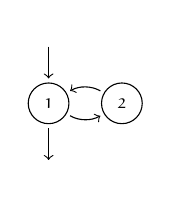
\begin{tikzpicture}
[
  every node/.style={
    font=\tiny
  },
  every initial by arrow/.style={
    shorten >=.5mm
  },
  every accepting by arrow/.style={
    shorten <=.5mm
  },
  entry above/.style={
    initial above,
    initial text=
  },
  exit below/.style={
    accepting below
  },
  bb/.style={
    circle,
    draw
  },
  tip/.style={
    shorten <=.5mm,
    shorten >=.5mm,
    ->,
    draw
  }
]

\node (entry) [bb,entry above,exit below] {$1$};
\node (body)  [bb,right=4mm of entry] {$2$};

\path [tip, bend right] (entry) edge (body);
\path [tip, bend right] (body) edge (entry);
\end{tikzpicture}

\end{block}

\column{.30\textwidth}
\begin{block}{Irreducible Loops}
\centering

% irreducible-loop.tex: irreducible loop shape.

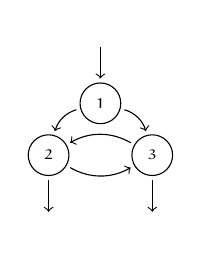
\begin{tikzpicture}
[
  every node/.style={
    font=\tiny
  },
  every initial by arrow/.style={
    shorten >=.5mm
  },
  every accepting by arrow/.style={
    shorten <=.5mm
  },
  entry above/.style={
    initial above,
    initial text=
  },
  exit below/.style={
    accepting below
  },
  bb/.style={
    circle,
    draw
  },
  tip/.style={
    shorten <=.5mm,
    shorten >=.5mm,
    ->,
    draw
  }
]

\node (entry)  [bb,entry above] {$1$};
\node (body-1) [bb,exit below,below left=4mm of entry] {$2$};
\node (body-2) [bb,exit below,below right=4mm of entry] {$3$};

\path [tip,bend right] (entry) edge (body-1);
\path [tip,bend left]  (entry) edge (body-2);

\path [tip,bend right] (body-1) edge (body-2);
\path [tip,bend right] (body-2) edge (body-1);
\end{tikzpicture}

\end{block}
\end{columns}

\bigskip
In LLVM the focus is on one kind of loop:

\begin{itemize}
\item natural loops
\end{itemize}
\end{frame}

\begin{frame}{Natural Loops}
A natural loop:

\begin{itemize}
\item has only one entry node -- \emph{header}
\item there is a back edge that enter the loop header
\end{itemize}

\vfill
Under this definition:

\begin{itemize}
\item the irreducible loop is not a natural loop
\item since LLVM consider only natural loops, the irreducible loop \alert{is not
      recognized} as a loop
\end{itemize}
\end{frame}

\begin{frame}{Loop Terminology}
Loops defined starting from back-edges:

\vfill
\begin{description}
\item[back-edge] edge entering loop header: $(3,1)$
\end{description}

\begin{columns}[t]
\column{.59\textwidth}
\begin{description}
\item[header] loop entry node: $1$
\item[body] nodes that can reach back-edge source node ($3$) without passing
            from back-edge target node ($1$) plus back-edge target node:
            $\{1 ,2, 3\}$
\end{description}
\column{.32\textwidth}
\vspace*{-1em}
\begin{block}{\small A loop}
\vspace*{-1em}

% loop-nodes.tex: loop terminology by picture.

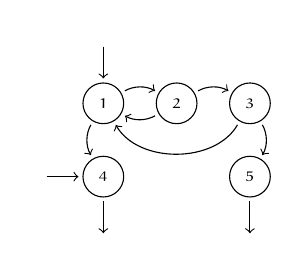
\begin{tikzpicture}
[
  every node/.style={
    font=\tiny
  },
  every initial by arrow/.style={
    shorten >=.5mm
  },
  every accepting by arrow/.style={
    shorten <=.5mm
  },
  entry above/.style={
    initial above,
    initial text=
  },
  entry left/.style={
    initial left,
    initial text=
  },
  exit below/.style={
    accepting below
  },
  bb/.style={
    circle,
    draw
  },
  tip/.style={
    shorten <=.5mm,
    shorten >=.5mm,
    ->,
    draw
  }
]

\node (entry)  [bb,entry above] {$1$};
\node (body-1) [bb,right=4mm of entry] {$2$};
\node (body-2) [bb,right=4mm of body-1] {$3$};

\node (exit-1) [bb,entry left,exit below,below=4mm of entry] {$4$};
\node (exit-2) [bb,exit below,below=4mm of body-2] {$5$};

\path [tip,bend left] (entry) edge (body-1);
\path [tip,bend left] (body-1) edge (body-2);

\path [tip,bend left]    (body-1) edge (entry);
\path [tip,bend left=60] (body-2) edge (entry);

\path [tip,bend right] (entry) edge (exit-1);
\path [tip,bend left]  (body-2) edge (exit-2);
\end{tikzpicture}

\end{block}


\end{columns}

\begin{description}
\item[exiting] nodes with a successor outside the loop: $\{1, 3\}$
\item[exit] nodes with a predecessor inside the loop: $\{4, 5\}$
\end{description}
\end{frame}

\begin{frame}{Loop Simplify}
Natural loops finding is the base pass \alert{identify} loops, but:

\begin{itemize}
\item some features are not analysis/optimization friendly
\end{itemize}

\vfill
The \texttt{loop-simplify} pass normalize natural loops:

\begin{columns}[t]
\column{.50\textwidth}
\begin{description}
\item[pre-header] the \alert{only predecessor} of \alert{header} node
\item[latch] the \alert{starting node} of the \alert{only back-edge}
\item[exit-block] ensures \alert{exits dominated} by loop \alert{header}
\end{description}

\column{.40\textwidth}
\begin{block}{Pre-header Insertion}
\centering

% pre-header.tex: adding pre-header.

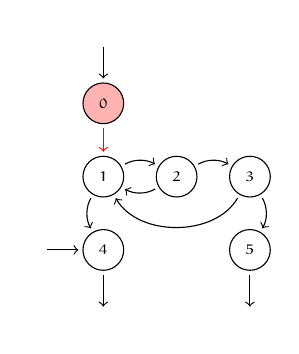
\begin{tikzpicture}
[
  every node/.style={
    font=\tiny
  },
  every initial by arrow/.style={
    shorten >=.5mm
  },
  every accepting by arrow/.style={
    shorten <=.5mm
  },
  entry above/.style={
    initial above,
    initial text=
  },
  entry left/.style={
    initial left,
    initial text=
  },
  exit below/.style={
    accepting below
  },
  bb/.style={
    circle,
    draw
  },
  tip/.style={
    shorten <=.5mm,
    shorten >=.5mm,
    ->,
    draw
  }
]

\node (pre-header) [bb,entry above,fill=red!30] {$0$};

\node (entry)  [bb,below=4mm of pre-header] {$1$};
\node (body-1) [bb,right=4mm of entry] {$2$};
\node (body-2) [bb,right=4mm of body-1] {$3$};

\node (exit-1) [bb,entry left,exit below,below=4mm of entry] {$4$};
\node (exit-2) [bb,exit below,below=4mm of body-2] {$5$};

\path [tip,color=red] (pre-header) edge (entry);

\path [tip,bend left] (entry) edge (body-1);
\path [tip,bend left] (body-1) edge (body-2);

\path [tip,bend left]    (body-1) edge (entry);
\path [tip,bend left=60] (body-2) edge (entry);

\path [tip,bend right] (entry) edge (exit-1);
\path [tip,bend left]  (body-2) edge (exit-2);
\end{tikzpicture}

\end{block}
\end{columns}
\end{frame}

\begin{frame}{Loop Simplify}{Example}
\begin{columns}[t]
\column{.45\textwidth}
\begin{block}{Latch Insertion}
\centering

% latch.tex: ensure only one back-edge.

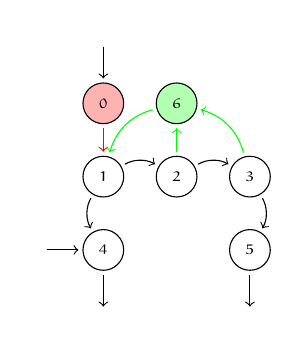
\begin{tikzpicture}
[
  every node/.style={
    font=\tiny
  },
  every initial by arrow/.style={
    shorten >=.5mm
  },
  every accepting by arrow/.style={
    shorten <=.5mm
  },
  entry above/.style={
    initial above,
    initial text=
  },
  entry left/.style={
    initial left,
    initial text=
  },
  exit below/.style={
    accepting below
  },
  bb/.style={
    circle,
    draw
  },
  tip/.style={
    shorten <=.5mm,
    shorten >=.5mm,
    ->,
    draw
  }
]

\node (pre-header) [bb,entry above,fill=red!30] {$0$};

\node (entry)  [bb,below=4mm of pre-header] {$1$};
\node (body-1) [bb,right=4mm of entry] {$2$};
\node (body-2) [bb,right=4mm of body-1] {$3$};
\node (latch)  [bb,above=4mm of body-1,fill=green!30] {$6$};

\node (exit-1) [bb,entry left,exit below,below=4mm of entry] {$4$};
\node (exit-2) [bb,exit below,below=4mm of body-2] {$5$};

\path [tip,color=red] (pre-header) edge (entry);

\path [tip,bend left] (entry) edge (body-1);
\path [tip,bend left] (body-1) edge (body-2);

\path [tip,color=green]            (body-1) edge (latch);
\path [tip,color=green,bend right] (body-2) edge (latch);
\path [tip,color=green,bend right] (latch) edge (entry);

\path [tip,bend right] (entry) edge (exit-1);
\path [tip,bend left]  (body-2) edge (exit-2);
\end{tikzpicture}

\end{block}

\column{.45\textwidth}
\begin{block}{Exit-block Insertion}
\centering

% exit-block.tex: ensure loop exit dominated by loop header.

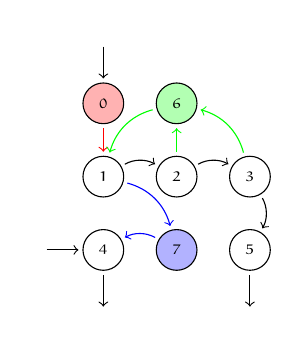
\begin{tikzpicture}
[
  every node/.style={
    font=\tiny
  },
  every initial by arrow/.style={
    shorten >=.5mm
  },
  every accepting by arrow/.style={
    shorten <=.5mm
  },
  entry above/.style={
    initial above,
    initial text=
  },
  entry left/.style={
    initial left,
    initial text=
  },
  exit below/.style={
    accepting below
  },
  bb/.style={
    circle,
    draw
  },
  tip/.style={
    shorten <=.5mm,
    shorten >=.5mm,
    ->,
    draw
  }
]

\node (pre-header) [bb,entry above,fill=red!30] {$0$};

\node (entry)  [bb,below=4mm of pre-header] {$1$};
\node (body-1) [bb,right=4mm of entry] {$2$};
\node (body-2) [bb,right=4mm of body-1] {$3$};
\node (latch)  [bb,above=4mm of body-1,fill=green!30] {$6$};

\node (exit-0) [bb,below=4mm of body-1,fill=blue!30] {$7$};
\node (exit-1) [bb,entry left,exit below,below=4mm of entry] {$4$};
\node (exit-2) [bb,exit below,below=4mm of body-2] {$5$};

\path [tip,color=red] (pre-header) edge (entry);

\path [tip,bend left] (entry) edge (body-1);
\path [tip,bend left] (body-1) edge (body-2);

\path [tip,color=green]            (body-1) edge (latch);
\path [tip,color=green,bend right] (body-2) edge (latch);
\path [tip,color=green,bend right] (latch) edge (entry);

\path [tip,bend left,color=blue]  (entry) edge (exit-0);
\path [tip,bend right,color=blue] (exit-0) edge (exit-1);
\path [tip,bend left]             (body-2) edge (exit-2);
\end{tikzpicture}

\end{block}
\end{columns}

\begin{itemize}
\item pre-header always executed before entering the loop
\item latch always executed before starting a new iteration
\item exit-blocks always executed after exiting the loop
\end{itemize}
\end{frame}

\begin{frame}{Loop-closed SSA}
Loop representation can be further normalized:

\begin{itemize}
\item \texttt{loop-simplify} normalize the \alert{shape} of the loop
\item nothing is said about loop definitions
\end{itemize}

\vfill
Keeping SSA form is expensive with loops:

\begin{itemize}
\item \texttt{lcssa} insert \llvminline{phi} instruction at loop boundaries for
      variables \alert{defined inside} the loop body and \alert{used outside}
\item this guarantees isolation between optimization performed inside and outside
      the loop
\item faster keeping IR into SSA form -- propagation of code changes outside the
      loop blocked by \llvminline{phi} instructions
\end{itemize}
\end{frame}

\begin{frame}{Loop-closed SSA}{Example}
\begin{block}{Linear Search}
\centering
\cinput{snippet/lcssa.c}
\end{block}

\vfill
The example is trivial:

\begin{itemize}
\item think about having large loop bodies
\item transformation becomes useful
\end{itemize}
\end{frame}

\begin{frame}{Loop-closed SSA}{Example}
\begin{block}{Before LCSSA}
\centering
\llvminput{snippet/before-lcssa.ll}
\end{block}
\vspace{\baselineskip}
\vfill
\end{frame}

\begin{frame}{Loop-closed SSA}{Example}
\begin{block}{After LCSSA}
\centering
\llvminput{snippet/after-lcssa.ll}
\end{block}
\vfill
\end{frame}

\begin{frame}{Induction Variables}
Some loop variables are \emph{special}:

\begin{itemize}
\item e.g. counters
\end{itemize}

\vfill
Generalization lead to \alert{induction variables}:

\begin{itemize}
\item \cinline{foo} is a loop induction variable if its successive values form
      an arithmetic progression:

      \begin{center}
      \cinline{foo = bar * baz + biz}
      \end{center}

      where \cinline{bar, biz} are
      loop-invariant~\footnote{Constants inside the loop}, and \cinline{baz} is
      an induction variable
\item \cinline{foo} is a \alert{canonical} induction variable if it is always
      incremented by a constant amount:

      \begin{center}
      \cinline{foo = foo + biz}
      \end{center}

      where \cinline{biz} is loop-invariant
\end{itemize}
\end{frame}

\begin{frame}{Induction Variable Simplification}
Canonical induction variables are used to \alert{drive} loop execution:

\begin{itemize}
\item given a loop, the \texttt{indvars} pass tries to find its canonical
      induction variable
\end{itemize}

\vfill
With respect to theory, LLVM canonical induction variable is:

\begin{itemize}
\item initialized to \llvminline{0}
\item incremented by \llvminline{1} at each loop iteration
\end{itemize}
\end{frame}

\begin{frame}{Normalization}{Wrap-up}
Normalization passes running order:

\begin{enumerate}
\item \texttt{mem2reg}: limit use of memory, increasing the effectiveness of
       subsequent passes
\item \texttt{loop-simplify}: canonicalize loop shape, lower burden of writing
      passes
\item \texttt{lcssa}: keep effects of subsequent loop optimizations local,
      limiting overhead of maintaining SSA form
\item \texttt{indvars}: normalize induction variables, highlighting the
      canonical induction variable
\end{enumerate}

\vfill
Other normalization passes available:

\begin{itemize}
\item try running \texttt{opt -help}
\end{itemize}
\end{frame}


% !TEX root = 02.tex

\section{Analysis Passes}


\begin{frame}{Checking Input Properties}
Analyses basically allow to:
\begin{itemize}
\item \alert{derive} information and properties of the input
\item \alert{verify} properties of input
\end{itemize}

\vfill
Keeping analyzed information updated is expensive:
\begin{itemize}
\item tuned algorithms update information when an optimization
      invalidates it
\item incrementally updating analyses are cheaper than recomputing them
\end{itemize}

\vfill
As an \alert{optimization}, many LLVM analysis supports incremental updates.
\end{frame}


\begin{frame}{Useful Analyses}
\begin{center}
We will see the following passes:\\
\bigskip
\begin{tabular}{ccc}
\toprule

\multicolumn{1}{c}{\textbf{Pass}}        &
\multicolumn{1}{c}{\textbf{Switch}}      &
\multicolumn{1}{c}{\textbf{Transitive}} \\

\midrule

Control flow graph  &
---       &
No                 \\

Dominator tree    &
\texttt{domtree}  &
No               \\

Post-dominator tree   &
\texttt{postdomtree}  &
No                   \\

Loop information  &
\texttt{loops}    &
Yes              \\

Scalar evolution           &
\texttt{scalar-evolution}  &
Yes                       \\

Alias analysis    &
---  &
Yes              \\

Memory SSA  &
\texttt{memoryssa}    &
Yes               \\

\bottomrule
\end{tabular}
\end{center}
\end{frame}


\begin{frame}{Requesting an Analysis}
\begin{center}
Your pass needs to tell the pass manager which analyses it needs!

\vfill
Transitive analyses:\\
\cppinline{llvm::AnalysisUsage::addRequiredTransitive<T>()}\\
\medskip
Non-transitive analyses: \\
\cppinline{llvm::AnalysisUsage::addRequired<T>()}\\

\vfill
For \alert{chained analyses}\footnote{Analyses that use the result of another analysis}, the \texttt{addRequiredTransitive} method
should be used instead of the \texttt{addRequired} method.\\
\medskip
{\small
This informs the PassManager that the transitively required pass
should be alive as long as the requiring pass is.}
\end{center}
\end{frame}


\subsection{Control Flow Graph}


\begin{frame}{Control Flow Graph}
The Control Flow Graph is implicitly maintained by LLVM:

\begin{itemize}
\item no specific pass to build it
\end{itemize}

\vfill
Recap:

\begin{itemize}
\item CFG for a function is a graph of basic blocks
\item a basic block is a list of instructions
\end{itemize}

\vfill
Functions and basic blocks act like containers:

\begin{itemize}
\item STL-like accessors: \cppinline{front()}, \cppinline{back()},
      \cppinline{size()}, \ldots
\item STL-like iterators: \cppinline{begin()}, \cppinline{end()}
	\begin{itemize}
	\item Warning for BBs: order of iteration $\neq$ order of execution!
	\end{itemize}
\end{itemize}

\vfill
Each contained element is aware of its container:

\begin{itemize}
\item \cppinline{getParent()}
\end{itemize}
\end{frame}


\begin{frame}{Control Flow Graph}{Walking}
Every CFG has an \alert{entry} basic block:

\begin{itemize}
\item the \alert{first} executed basic block
\item it is the \alert{root/source} of the graph
\item get it with \cppinline{llvm::Function::getEntryBlock()}
\end{itemize}

\vfill
At the end of a basic blocks there's always a \alert{terminator} instruction:
\begin{itemize}
\item \llvminline{ret}, \llvminline{br}, \llvminline{switch}, \llvminline{unreachable}, \ldots
\end{itemize}

\vfill
More than one \alert{exit} block can be present in a function:

\begin{itemize}
\item they are the \alert{leaves/sinks} of the graph
\item their terminator instructions are always \llvminline{ret}s
\begin{enumerate}
\item \cppinline{llvm::BasicBlock::getTerminator()}
\item check the opcode of the terminator
\end{enumerate}
\end{itemize}
\end{frame}


\begin{frame}{Side Note}{Casting Framework}
For performance reasons, a custom casting framework is used:

\begin{itemize}
\item you cannot use \cppinline{static\_cast} and \cppinline{dynamic\_cast} with
      types/classes provided by LLVM
\end{itemize}

\begin{block}{LLVM Casting Functions}
\centering
\medskip
\begin{tabular}{rl}

Static cast of \cppinline{Y*} to \cppinline{X}  &
\cppinline{X *llvm::cast<X>(Y *)}                \\

Dynamic cast of \cppinline{Y*} to \cppinline{X}  &
\cppinline{X *llvm::dyn\_cast<X>(Y *)}            \\

Is \cppinline{Y*} an instance of \cppinline{X}?  &
\cppinline{bool llvm::isa<X>(Y *)} \\

\end{tabular}
\smallskip
\end{block}

Example:

\begin{itemize}
\item is \cppinline{BB} a sink?\\
      \cppinline{llvm::isa<llvm::ReturnInst>(BB.getTerminator())}
\end{itemize}
\end{frame}


\begin{frame}{Control Flow Graph}{Basic Blocks}
Every basic block \cppinline{BB} has one or more\footnote{see include/llvm/IR/CFG.h}:

\begin{description}[predecessors]
\item[predecessors] from \cppinline{pred\_begin(BB)} to
      \cppinline{pred\_end(BB)}
\item[successors] from \cppinline{succ\_begin(BB)} to
      \cppinline{succ\_end(BB)}
\end{description}

\vfill
Other convenience methods available in \cppinline{llvm::BasicBlock}:

\begin{itemize}
\item useful getters
\begin{itemize}
\item \cppinline{BasicBlock *getUniquePredecessor()}
\item \ldots
\end{itemize}
\item moving a basic block
\begin{itemize}
\item      \cppinline{moveBefore(llvm::BasicBlock *)}
\item      \cppinline{moveAfter(llvm::BasicBlock *)}
\end{itemize}
\item split a basic block:
\begin{itemize}
\item      \cppinline{splitBasicBlock(llvm::BasicBlock::iterator)}
\end{itemize}
\item \ldots
\end{itemize}
\end{frame}


\begin{frame}{Control Flow Graph}{Instructions}
The \cppinline{llvm::Instruction} class defines common operations: \\
\medskip
\begin{itemize}
\item getting an operand
\begin{itemize}
\item \cppinline{getOperand(unsigned)}
\end{itemize}
\end{itemize}
\vfill
Subclasses provide specialized accessors: \\
\medskip
\begin{itemize}
\item the \llvminline{load} instruction takes as operand the pointer to the memory to be loaded:
\begin{itemize}
\item      \cppinline{llvm::LoadInst::getPointerOperand()}
\end{itemize}
\end{itemize}
\end{frame}


\begin{frame}{Instructions}{Creating New Instructions}
Instructions are created using:

\begin{itemize}
\item constructors
\begin{itemize}
\item \cppinline{llvm::LoadInst::LoadInst(...)}
\end{itemize}
\item factory methods
\begin{itemize}
\item \cppinline{llvm::GetElementPtrInst::Create(...)}
\end{itemize}
\item the helper class \cppinline{llvm::IRBuilder}
\begin{itemize}
\item \cppinline{llvm::IRBuilder<> builder(insPoint);}\\
\cppinline{builder.CreateAdd(...);}
\end{itemize}
\end{itemize}
\vfill
\alert{Interface is not homogeneous!}\\
Some instructions support all methods, others support only one.
\end{frame}


\begin{frame}{Instructions}{Inserting New Instructions}


\vfill
Instructions can be inserted:
\vfill
\begin{itemize}
\item automatically by \cppinline{IRBuilder}
\begin{itemize}
\item insertion point is given at \cppinline{IRBuilder} instantiation
\end{itemize}
\bigskip
\item manually by appending to a basic block
\item manually by inserting after/before another instruction
\end{itemize}
\vfill
\end{frame}


\begin{frame}{From Control Flow to Data Flow}{Definitions and Uses}
In LLVM, the data flow generated by the various instructions is represented by a simple hierarchy:

\begin{description}[valueMMM]
\item[value] something that can be used: \cppinline{llvm::Value}
\item[user] something that can use: \cppinline{llvm::User}
\item[use] the link between the \alert{value} and the \alert{user}: \cppinline{llvm::Use}
\end{description}
\medskip
A value is a \alert{definition}:

\begin{itemize}
\item Visiting where a definition is used:
\begin{itemize}
\item \cppinline{llvm::Value::use\_begin()}, \cppinline{llvm::Value::use\_end()}
\end{itemize}
\end{itemize}
\medskip
An user accesses \alert{definitions}:

\begin{itemize}
\item Visiting the definitions that are used:
\begin{itemize}
\item \cppinline{llvm::User::op\_begin()}, \cppinline{llvm::User::op\_end()}
\end{itemize}
\end{itemize}
\medskip

\end{frame}


\begin{frame}{From Control Flow to Data Flow}{Instructions are Values}
\vfill
\begin{itemize}
\item \cppinline{llvm::Value} inherits from \cppinline{llvm::User}
\item \cppinline{llvm::Instruction} inherits from \cppinline{llvm::Value}
\begin{itemize}
\normalsize
\item[$\Rightarrow$] The value produced by the instruction is\\the \alert{instruction itself}!
\end{itemize}
\end{itemize}

\begin{block}{Example}
\begin{center}
\llvminline{\%6 = load i32, i32* \%1, align 4}\\
\medskip
The \llvminline{load} is described by an instance of \cppinline{llvm::Instruction}. \\
That instance also represents the \llvminline{\%6} variable. \\
\end{center}
\end{block}

\begin{center}
Not all instances of \cppinline{llvm::Value} are also \cppinline{llvm::Instruction}s!\\
\smallskip
{\small i.e. function arguments}

\end{center}
\vfill
\end{frame}


\begin{frame}{From Control Flow to Data Flow}{Value Typing}
Every \cppinline{llvm::Value} is typed:

\begin{itemize}
\item use \cppinline{llvm::Value::getType()} to get the type
\end{itemize}

\vfill
Since every instruction is a value:

\begin{itemize}
\item instructions are typed
\end{itemize}

\vfill
\begin{block}{Example}
\begin{center}
\llvminline{\%6 = load i32, i32* \%1, align 4}\\
\medskip
The type of the \llvminline{\%6} variable is the type of the return value of the \llvminline{load} instruction, \llvminline{i32}\\
\end{center}
\end{block}
\end{frame}


%\begin{frame}{From Control Flow to Data Flow}{Instructions are like functions}
%\vfill
%\vfill
%\begin{columns}[t]
%\column{.45\textwidth}
%Functions:
%
%\begin{itemize}
%\item used by call sites
%\item uses formal parameters
%\end{itemize}
%
%\column{.45\textwidth}
%Instructions:
%
%\begin{itemize}
%\item define an SSA value
%\item uses operands
%\end{itemize}
%\end{columns}
%
%\vfill
%\vfill
%\end{frame}


\subsection{Dominance Trees}


\begin{frame}{Dominance Trees}
Dominance trees answer to control-related queries:\\

\vfill
\begin{columns}[onlytextwidth]
\column{.475\textwidth}
\begin{centering}
is \texttt{A} executed \alert{before} \texttt{B}?\\
$\Downarrow$\\
\cppinline{llvm::DominatorTree}\\
\end{centering}

\column{.525\textwidth}
\begin{centering}
is \texttt{A} executed \alert{after} \texttt{B}?\\
$\Downarrow$\\
\cppinline{llvm::PostDominatorTree}\\
\end{centering}
\end{columns}

\vfill
The interfaces of these two trees is mostly the same:

\begin{itemize}
\item \cppinline{bool dominates(A, B)}
\item \cppinline{bool properlyDominates(A, B)}
\end{itemize}

\cppinline{A} and \cppinline{B} are either
\cppinline{llvm::BasicBlock}s or
\cppinline{llvm::Instruction}s

\vfill
By using \texttt{opt}, it is possible to show the trees:

\begin{itemize}
\item \aligntext{\texttt{-view-postdom},}{\texttt{-view-dom},} \texttt{-dot-dom}
\item \aligntext{\texttt{-view-postdom},}{\texttt{-view-postdom},} \texttt{-dot-postdom}
\end{itemize}
\end{frame}


\subsection{Loop Information}


\begin{frame}{Loop Information}
Loop information is represented using two classes:

\begin{description}[\texttt{llvm::LoopInfo}]
\item[\texttt{llvm::LoopInfo}]
			The result of \cppinline{llvm::LoopAnalysis},\\
			performed on a given function.
\item[\texttt{llvm::Loop}]
			Represents a single loop in a function.\\
			Contained inside a \texttt{llvm::LoopInfo}.
\end{description}

\vfill
Using \cppinline{llvm::LoopInfo} it is possible:

\begin{itemize}
\item navigate through top-level loops:
\begin{itemize}
\item \cppinline{llvm::LoopInfo::begin()}
\item \cppinline{llvm::LoopInfo::end()}
\end{itemize}
\item get the loop for a given basic block:
\begin{itemize}
\item \cppinline{llvm::LoopInfo::operator[](llvm::BasicBlock *)}
\end{itemize}
\end{itemize}
\end{frame}


\begin{frame}{Loop Information}{Nesting Tree}
Loops are represented as a \alert{tree}:\\
\begin{columns}
\column{.6\textwidth}
\begin{block}{Source\vphantom{Loop Nest}}
\cinput[\tt\fontsize{7.5pt}{7.5pt}\selectfont]{snippet/loop-nest.c}
\end{block}
\column{.3\textwidth}
\begin{block}{Loop Hierarchy}
\centering

% loop-nest.tex: a simple loop nest.

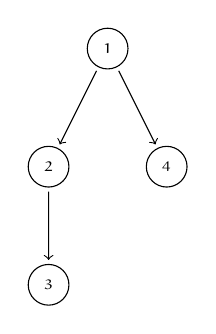
\begin{tikzpicture}
[
  every node/.style={
    font=\tiny
  },
  loop/.style={
    circle,
    draw
  },
  tip/.style={
    shorten <=.5mm,
    shorten >=.5mm,
    ->,
    draw
  },
  level 1/.style={
    edge from parent/.style=tip
  },
]

\node [loop] {$1$}
  child { node [loop] {$2$}
    child { node [loop] {$3$}}
  }
  child { node [loop] {$4$}};
\end{tikzpicture}

\end{block}
\end{columns}
\vfill
\begin{description}[children loops]
\item[children loops] \cppinline{llvm::Loop::begin()},
      \cppinline{end()}
\item[parent loop] \cppinline{llvm::Loop::getParentLoop()}
\end{description}
\end{frame}


\begin{frame}{Loop Information}{Query Loops}
Accessors for important nodes:

\begin{description}
\item[pre-header] \cppinline{llvm::Loop::getLoopPreheader()}
\item[header] \cppinline{llvm::Loop::getHeader()}
\item[latch] \cppinline{llvm::Loop::getLoopLatch()}
\item[exiting] \cppinline{llvm::Loop::getExitingBlock()}, \\
               \cppinline{llvm::Loop::getExitingBlocks(...)}
\item[exit] \cppinline{llvm::Loop::getExitBlock()} \\
            \cppinline{llvm::Loop::getExitBlocks(...)}
\end{description}

\vfill
The list of all BBs in the loop is accessible via:

\begin{description}
\item[iterators] \cppinline{llvm::Loop::block\_begin()}, \\
                 \cppinline{llvm::Loop::block\_end()}
\item[vector]
      \texttt{\addfontfeature{LetterSpace=-5}std::vector<BasicBlock *> \&Loop::getBlocks()}
\end{description}
\end{frame}


\subsection{Scalar Evolution}


\begin{frame}{Scalar Evolution}
The \alert{SC}alar \alert{EV}olution pass analyzes scalar
expressions inside loops.

\begin{itemize}
\item all expressions are categorized and represented uniformly
\item is capable of handling \alert{general induction variables}
\item also useful outside of loops
\item \texttt{opt} flags: \texttt{-analyze -scalar-evolution}
\end{itemize}

\vfill
\begin{columns}[onlytextwidth]
\column{.67\textwidth}
\begin{block}{Example}
\llvminput[\tt\scriptsize]{snippet/basic-scev.ll}
\end{block}

\column{.30\textwidth}
SCEV for \llvminline{\%i.0}:

\begin{itemize}
\item initial value $0$
\item incremented \\by $1$ at each iteration
\item final value $10$
\end{itemize}
\end{columns}
\end{frame}


\begin{frame}{Scalar Evolution}{Example}
\begin{columns}
\column{.55\textwidth}
\begin{block}{Source}
\cinput[\tt\small]{snippet/nested-scev.c}
\end{block}

\column{.35\textwidth}
SCEV \llvminline{\{A,B,C\}<\%D>}:

\begin{itemize}
\item \llvminline{A} starting value
\item \llvminline{B} operator
\item \llvminline{C} stride
\item \llvminline{D} loop head BB
\end{itemize}

\llvminline{\{0,+,1\}=0+1+1+1+}\ldots

\end{columns}

\vfill
\begin{block}{Induction Variables}
\centering
\llvminput[\tt\small]{snippet/nested-scev-induction.ll}
\end{block}
\end{frame}


\begin{frame}{Scalar Evolution}{More than Induction Variables}
The scalar evolution framework manages \alert{any scalar expression}:

\begin{block}{Pointer SCEVs in two nested loops}
\centering
\llvminput[\tt\footnotesize]{snippet/nested-scev-pointer.ll}
\end{block}

\vfill
SCEV is an analysis used by many common optimizations
\begin{itemize}
\small
\item induction variable substitution
\item strength reduction
\item vectorization
\item \ldots
\end{itemize}
\end{frame}


\begin{frame}{Scalar Evolution}{SCEVs Design}
SCEVs are modeled by the \cppinline{llvm::SCEV} class:

\begin{itemize}
\item a subclass for each kind of SCEV: e.g. \cppinline{llvm::SCEVAddExpr}
\item instantiation disabled
\end{itemize}

\vfill
A SCEV actually is a tree of SCEVs:

\begin{itemize}
\item \llvminline{\{(80 + \%bar),+,80\}} =
\begin{itemize}
\item			\llvminline{\{\%1,+,80\}}
\item     \llvminline{\%1 = 80 + \%bar}
\end{itemize}
\end{itemize}

Tree leaves:

\begin{description}
\item[constant] \cppinline{llvm::SCEVConstant}: e.g. \llvminline{80}
\item[unknown\footnote{Not further splittable}] \cppinline{llvm::SCEVUnknown}:
                                                 e.g. \llvminline{\%bar}
\end{description}

\vfill
SCEV tree explorable through the visitor pattern:

\begin{itemize}
\item \cppinline{llvm::SCEVVisitor}
\end{itemize}
\end{frame}


\begin{frame}{Scalar Evolution}{Analysis Interface}
\centering
The \cppinline{llvm::ScalarEvolutionAnalysis} pass computes all the
SCEVs for a given \cppinline{llvm::Function}.
\vfill
\centering
The \cppinline{llvm::ScalarEvolution} instance produced by the pass
provides the following services:
\vfill
\begin{itemize}
\item get the SCEV representing a value:
\begin{itemize}
\item      \cppinline{getSCEV(llvm::Value *)}
\end{itemize}
\vfill
\item get important SCEVs from other structures or SCEVs:
\begin{itemize}
\item      \cppinline{getBackedgeTakenCount(llvm::Loop *)}
\item      \cppinline{getPointerBase(llvm::SCEV *)}
\item      \ldots
\end{itemize}
\vfill
\item create new SCEVs explicitly:
\begin{itemize}
\item \cppinline{getConstant(llvm::ConstantInt *)}
\item \cppinline{getAddExpr(llvm::SCEV *, llvm::SCEV *)}
\item \ldots
\end{itemize}
\end{itemize}
\end{frame}


\subsection{Alias Analysis}


\begin{frame}{Alias Analysis}
Let $X$ be an instruction accessing a memory location:

\begin{itemize}
\item is there another instruction accessing the same location?
\end{itemize}

\vfill
Alias analysis tries to answer the question:

\begin{description}
\item[application] optimization of memory operations
\item[problem] often fails
\end{description}

\vfill
Different algorithms are available for alias analysis:

\begin{itemize}
\item common interface: \cppinline{llvm::AAResults}
\item base implementation: basic alias analysis (\texttt{basicaa})
\end{itemize}

\begin{block}{Requiring Alias Analysis}
\centering
\cppinput{snippet/requiring-alias-analysis.cpp}
\end{block}
\end{frame}


\begin{frame}{Alias Analysis}{Memory Representation}
\begin{columns}
\column{.45\textwidth}
\begin{block}{Source}
\centering
\llvminput[\tt\footnotesize]{snippet/memory-locations.ll}
\end{block}

\centering
Basic building block:\\\texttt{llvm::MemoryLocation}\\
\medskip
Encapsulates a tuple:\\(\alert{address}, \alert{size})\\
\medskip
Can be computed from a \texttt{llvm::Value}

\column{.45\textwidth}
\begin{block}{Distinct Locations}
\centering

% alias-analysis-distinct.tex: different locations.

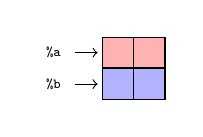
\begin{tikzpicture}
[
  every node/.style={
    font=\tiny
  },
  location/.style={
    rectangle split,
    rectangle split parts=2,
    rotate=90,
    draw
  },
  location-a/.style={
    location,
    rectangle split part fill={
      red!30,
      red!30
    }
  },
  location-b/.style={
    location,
    rectangle split part fill={
      blue!30,
      blue!30
    }
  },
  tip/.style={
    shorten <=.5mm,
    shorten >=.5mm,
    ->,
    draw
  }
]

\matrix [column sep=4mm]
{
\node (a) {\llvminline{\%a}}; & \node (a-loc) [location-a] {}; \\
\node (b) {\llvminline{\%b}}; & \node (b-loc) [location-b] {}; \\
};

\path [tip] (a) edge (a-loc.north);
\path [tip] (b) edge (b-loc.north);
\end{tikzpicture}

\end{block}

\begin{block}{Overlapping Locations}
\centering

% alias-analysis-overlapping.tex: overlapping locations.

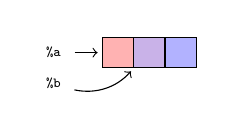
\begin{tikzpicture}
[
  every node/.style={
    font=\tiny
  },
  location/.style={
    rectangle split,
    rectangle split parts=3,
    rectangle split part fill={
      red!30,
      red!30!blue!30,
      blue!30
    },
    rotate=90,
    draw
  },
  tip/.style={
    shorten <=.5mm,
    shorten >=.5mm,
    ->,
    draw
  }
]

\matrix [column sep=4mm]
{
\node (a) {\llvminline{\%a}}; & \node (loc) [location] {}; \\
\node (b) {\llvminline{\%b}}; &                            \\
};

\path [tip]           (a) edge (loc.north);
\path [tip,bend right] (b) edge (loc.text split west);
\end{tikzpicture}

\end{block}

\begin{block}{Same Location}
\centering

% alias-analysis-same.tex: same location.

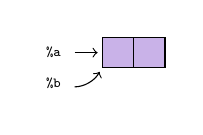
\begin{tikzpicture}
[
  every node/.style={
    font=\tiny
  },
  location/.style={
    rectangle split,
    rectangle split parts=2,
    rectangle split part fill={
      red!30!blue!30,
      red!30!blue!30
    },
    rotate=90,
    draw
  },
  tip/.style={
    shorten <=.5mm,
    shorten >=.5mm,
    ->,
    draw
  }
]

\matrix [column sep=4mm]
{
\node (a) {\llvminline{\%a}}; & \node (loc) [location] {}; \\
\node (b) {\llvminline{\%b}}; &                            \\
};

\path [tip]            (a) edge (loc.north);
\path [tip,bend right] (b) edge (loc.north west);
\end{tikzpicture}

\end{block}

\end{columns}
\end{frame}


\begin{frame}{Alias Analysis}{Basic Interface}
Given two memory locations $X$, $Y$, the alias analyzer classifies them:\\
\vfill
\begin{itemize}
\item \texttt{\textbf{llvm::AliasResult::NoAlias}}\\
			$X$ and $Y$ \alert{are
      different} memory locations
\vfill
\item \texttt{\textbf{llvm::AliasResult::MustAlias}}\\
			$X$ and $Y$ \alert{are equal}
      -- i.e. they points to the same address
\vfill
\item \texttt{\textbf{llvm::AliasResult::PartialAlias}}\\
			$X$ and $Y$
      \alert{partially overlap} -- i.e. they points to different addresses,
      but the pointed memory areas partially overlap
\vfill
\item \texttt{\textbf{llvm::AliasResult::MayAlias}}\\
			\alert{unable to compute}
      aliasing information -- i.e. $X$ and $Y$ can be different locations,
      or $X$ can be a complete/partial alias of $Y$
\end{itemize}

\vfill
Queries performed using:
\begin{itemize}
\item \cppinline{llvm::AAResults::alias(X, Y)}
\end{itemize}
\end{frame}


\begin{frame}{Alias Analysis}{Basic Interface}
A different categorization involves whether an instruction $I$
\alert{reads and/or modifies} a memory location $X$:\\
\vfill
\begin{itemize}
\item \texttt{\textbf{llvm::ModRefInfo::NoModRef}}\\
			The access neither references nor modifies the value stored in $X$
\vfill
\item \texttt{\textbf{llvm::ModRefInfo::Ref}}\\
			The access may reference the value stored in $X$ 
\vfill
\item \texttt{\textbf{llvm::ModRefInfo::Mod}}\\
			The access may modify the value stored in $X$ 
\vfill
\item \texttt{\textbf{llvm::ModRefInfo::ModRef}}\\
			The access may reference and may modify the value stored in $X$
\end{itemize}

\vfill
Queries performed using:
\begin{itemize}
\item \cppinline{llvm::AAResults::getModRefInfo(I, X)}
\end{itemize}
\end{frame}


\begin{frame}{Alias Analysis}{Mid-level Interface}
\begin{center}
This interface is very low-level!\\
\smallskip
What if we wanted to compute all aliases of a single value $X$?\\
\vfill
To do this, LLVM provides the \cppinline{llvm::AliasSet} class:

\begin{columns}
\column{0.75\textwidth}
\begin{enumerate}
\item instantiate a new \cppinline{llvm::AliasSetTracker}\\
			starting from \cppinline{llvm::AAResults}\footnotemark[1]
\item it builds (one or more) \cppinline{llvm::AliasSet}
\end{enumerate}
\end{columns}

\footnotetext[1]{\cppinline{using llvm::AliasAnalysis = llvm::AAResults\;}}
\vfill
For a given location $X$, a \cppinline{llvm::AliasSet}:

\begin{columns}
\column{0.6\textwidth}
\begin{itemize}
\item contains all locations aliasing with $X$
\end{itemize}
\end{columns}
\vfill
\end{center}
\end{frame}


\begin{frame}{Alias Analysis}{Alias Set Memory Accesses}
Alias sets return memory reference and aliasing information just like
the low-level interface.
\vfill
\alert{Warning:} This information is \alert{less precise}, 
as it is derived by \alert{conservatively aggregating}
more detailed data!

\vfill
\begin{itemize}
\item \texttt{\textbf{bool llvm::AliasSet::isRef()}}\\
			memory accessed in read-mode -- e.g. a
      \llvminline{load} is inside the set
\item \texttt{\textbf{bool llvm::AliasSet::isMod()}}\\
			memory accessed in write-mode -- e.g. a
      \llvminline{store} is inside the set
\vfill
\item \texttt{\textbf{bool llvm::AliasSet::isMustAlias()}}\\
			all pointers in the set \texttt{MustAlias} with each other
\item \texttt{\textbf{bool llvm::AliasSet::isMayAlias()}}\\
			at least one pair of pointer is not a \texttt{MustAlias} pair
\vfill
\end{itemize}
\end{frame}


\begin{frame}{Alias Analysis}{Mid-level Interface}
\begin{center}
Entry point is\\
\cppinline{llvm::AliasSetTracker::getAliasSetFor(...)}\\
\medskip
Only argument is a reference to\\
\cppinline{llvm::MemoryLocation}
\vfill
Once you have the \cppinline{llvm::AliasSet} you can inspect
the list of memory locations in it with the standard C++ iterator pattern:\\
\medskip
\cppinline{size()}, \cppinline{begin()}, \cppinline{end()}
\end{center}
\vfill
\end{frame}


\subsection{Memory SSA}


\begin{frame}{Memory SSA}{Alias Analyzer High-level Interface}
The \cppinline{llvm::MemorySSAAnalysis} pass wraps alias analysis to answer
queries in the following form:

\begin{itemize}
\item let \llvminline{\%foo} be an instruction accessing memory. Which
      preceding instructions does \llvminline{\%foo} depends on?
\end{itemize}

\vfill
This is done by representing all memory accesses in a\\\alert{SSA-like form}:
\begin{itemize}
\item \llvminline{store}-like instructions become \alert{definitions} (\llvminline{MemoryDef})
\item \llvminline{load}-like instructions become \alert{uses} (\llvminline{MemoryUse})
\item \llvminline{store}s to the same location in parallel CFG branches become \alert{phi}s (\llvminline{MemoryPhi})
\end{itemize}
\end{frame}


\begin{frame}{Memory Dependence Analysis}{APIs}
MemorySSA ``instructions'' are owned by \cppinline{llvm::MemorySSA} objects.\\
\bigskip
They are \alert{overlaid} on top of the normal CFG. \\
\smallskip
\begin{itemize}
\item \cppinline{AccessList *getBlockAccesses(BasicBlock *)}
\item \cppinline{DefsList *getBlockDefs(BasicBlock *)}
\end{itemize}
\bigskip
This basic interface is very \alert{hard to use}:\\
\smallskip
\begin{itemize}
\item \cppinline{llvm::MemorySSAWalker} provides support for the most common query
\item \cppinline{MemoryAccess *getClobberingMemoryAccess(...)}
\begin{itemize}
\item Returns the nearest dominating memory access that clobbers the
same memory location given.
\end{itemize}
\end{itemize}
\end{frame}


% !TEX root = main.tex

\section{Conclusion}


\begin{frame}{Conclusion}
We have seen:
\begin{itemize}
\item On which principles LLVM-MCA is based
\item How to use LLVM-MCA and how \alert{not} to use it
\item Which results can be achieved and what other factors 
	influence the speed at which your code runs
\item How LLVM-MCA is implemented and some hints on where to look
	if you want to expand or improve it
\end{itemize}
\bigskip
Have fun optimizing your programs!
\end{frame}


\begin{frame}[plain]{}
\Huge\centering
Thank You!\\
\bigskip
\normalsize
Questions?
\end{frame}




\section{Bibliography}
\begin{frame}[allowframebreaks]{Bibliography}
\nocite{*}
\bibliographystyle{unsrt}
\bibliography{bibliography-2}
\end{frame}
\end{document}
